\documentclass[onecolumn]{article}
%\usepackage{url}
%\usepackage{algorithmic}
\usepackage[a4paper]{geometry}
\usepackage{datetime}
\usepackage[margin=2em, font=small,labelfont=it]{caption}
\usepackage{graphicx}
\usepackage{mathpazo} % use palatino
\usepackage[scaled]{helvet} % helvetica
\usepackage{microtype}
\usepackage{amsmath}
\usepackage{subfigure}
\usepackage{float}
\documentclass[10pt,a4paper]{article}
\usepackage[demo]{graphicx}
\usepackage{subfig}
\usepackage{hyperref}
\usepackage[defaultfam,tabular,lining]{montserrat}

% Letterspacing macros
\newcommand{\spacecaps}[1]{\textls[200]{\MakeUppercase{#1}}}
\newcommand{\spacesc}[1]{\textls[50]{\textsc{\MakeLowercase{#1}}}}

\title{\spacecaps{Data Mining Final Project \\ Image processing to predict as cat or dog}\\ \normalsize \spacesc{CENG 3521, DATA MINING} }

\author{Team Name: Petbenders \\ --------------------------------- \\ Furkan Baldır \\ Mehmet Pekcan}
%\date{\today\\\currenttime}
\date{Report date: \today}

\begin{document}
\maketitle

\section*{Abstract}
In this project, the goal is predicting as cat or dog for given image. To train data, the Support Vector Machine model was created with using Python language. We did single and multiple predict operations to get results to calculate accuracy and also get the exact result which is cat or dog. On the other hand of project, there are front end part written with javascript library which is React, and API part written with Python again. 

\section{Introduction}
This project can work on local server as a web application. Also it can work on command line by using Python file.
% Buraya direkt ekran görüntüsü gelecek

\subsection{Goal}
The goal of this project is that using machine learning algorithm to make image processing. Generally, image processing projects made with using deep learning algorithms to get high accuracy values. However, machine learning algorithm can do the same things with less accuracy. This project aims to calculate accuracy value with using the SVC(Support Vector Machine) algorithm.
\newline
\newline
On the other hand, in this project, it is aimed that the end user can make predictions. To do that, our project deployed on web server to upload any image and to predict the animal. We used Javascript language to make a modern progressive web app to run this project. 

\subsection{Used Programming Languages}
- Python 3.8.7
\newline
- Javascript

\subsection{Used Libraries}
\boldsymbol{Python} \\ ------------------ \\ 
\textbf{Flask\_Cors 3.0.10}: To make request to api without crossorigin problem. \\ 
\textbf{Flask 1.1.2}: To create and deploy an API. \\ 
\textbf{Numpy 1.19.5} To convert image to mathematical array. \\
\textbf{Pillow 8.1.0} To open and to manipulate images. \\
\textbf{Scikit\_learn 0.24.1} To using Support Vector Machine algorithm. \\

\newline
\newline

\boldsymbol{Javascript} \\ ------------------ \\
\textbf{React}: To build Progrssive Web App \\
\textbf{Redux}: To handle app data on central place  \\
\textbf{Redux Saga}: To handle asynchronous actions like API request \\
\textbf{Redux Sauce}: To handle better and understandable with Saga pattern  \\
\textbf{Reselect}: To handle data without side effects \\
\textbf{Styled Components}: To handle styles better maintainable way when app grows \\
\textbf{Immer}: To handle saving data to Redux more clear way \\


\section{Preparing the Datasets}
This project needs a trained machine learning model to predict a result of given image. That's why there are some datasets used in this project.
\subsection{Training Dataset}
This is our training dataset. This dataset completely used for training, not testing.
\newline
\href{https://www.kaggle.com/chetankv/dogs-cats-images}{Training Dataset}
\newline
\newline
To use these dataset in this project, the images should convert to numpy arrays to use in our machine learning algorithms. That's why in source code, \boldsymbol{backend/training\_model\_creation.py} script has \boldsymbol{pick\_training\_data()} function to store dataset as "data.pickle".

\subsection{Testing Dataset}
This is our testing data. This dataset completely used for testing, not training.
\newline
\href{https://www.kaggle.com/kushleshkumar/cats-and-dogs}{Testing Dataset}
\newline
\newline
To use these dataset in this project, the images should convert again to numpy arrays to use in our machine learning algorithms. That's why in source code, \boldsymbol{backend/training\_model\_creation.py} script has \boldsymbol{pick\_test\_data()} function to store dataset as "test.pickle".

\section{Creating Machine Learning Model and Predicting}
In this project, we used Support Vector Machine algorithm that it exists in scikit-learn Python module to create machine learning model. In this project, our goal is creating a machine learning model, storing the model as a file, then using the file as a model while we are predicting an image.

\subsection{Converting Images to Numpy Array}
Firstly, images needs to be opened. To do that, \boldsymbol{Pillow} module used. Then, opened images converted to numpy array with using \boldsymbol{numpy} module.

\subsection{Creating Machine Learning Model}
To do that, from scikit-learn SVC() which is Support Vector Machine Classifier used to fit a model. In source code, \boldsymbol{backend/training\_model\_creation.py} has \boldsymbol{train\_data()} function.

\subsection{Storing Machine Learning Model}
To do that, \boldsymbol{Pickle} module used. When fitting the model finished, \boldsymbol{backend/file\_management.py} script used to call \boldsymbol{save\_file(filename, data)} function to save model as 'model.sav'.

\subsection{Predicting a Given Image}
The final part is predicting a given image. To do that, \boldsymbol{backend/predict.py} script used to call \boldsymbol{predict(img\_path)} function to get predicted result. It returns an integer(cat is 0, dog is 1)

\section{Bridge of Backend and Frontend: API}
To make a better user experience we should move our program from command line interfaces to graphical user interfaces. The first condition to do this movement, we created an API server using Flask. Its duty is basically take the request comes from frontend service then send it to our backend service.

\begin{figure}[H]
\centering
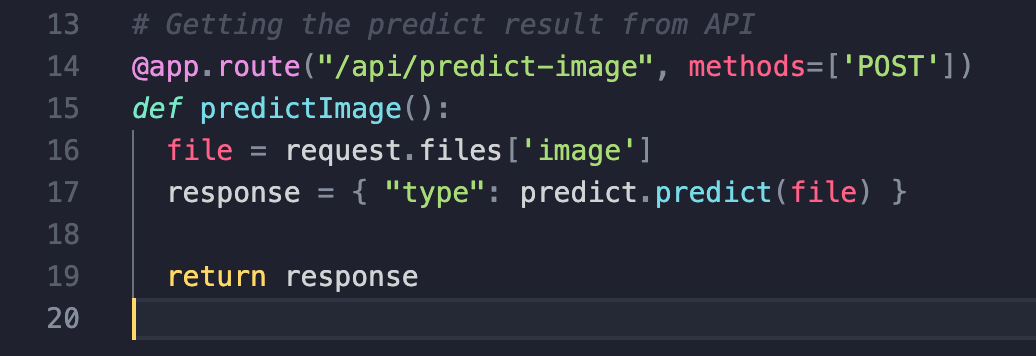
\includegraphics[scale=0.30]{api.png}
\caption{Predict route}
\end{figure}

Our API takes the image upload request with file data, then makes a backend call then return it as a JSON.

\section{Frontend}
As we mentioned previous section, the way of building a better user experience is passing to showing graphical interfaces to user. Not command line interface. So with this rule, we implemented a Progressive Web App that takes power of React. That is the better way to take image from user and showing the predicted class. We don't mention the whole frontend logic here because it is not the information that directly relevant about this project.

\begin{figure}[H]
\centering
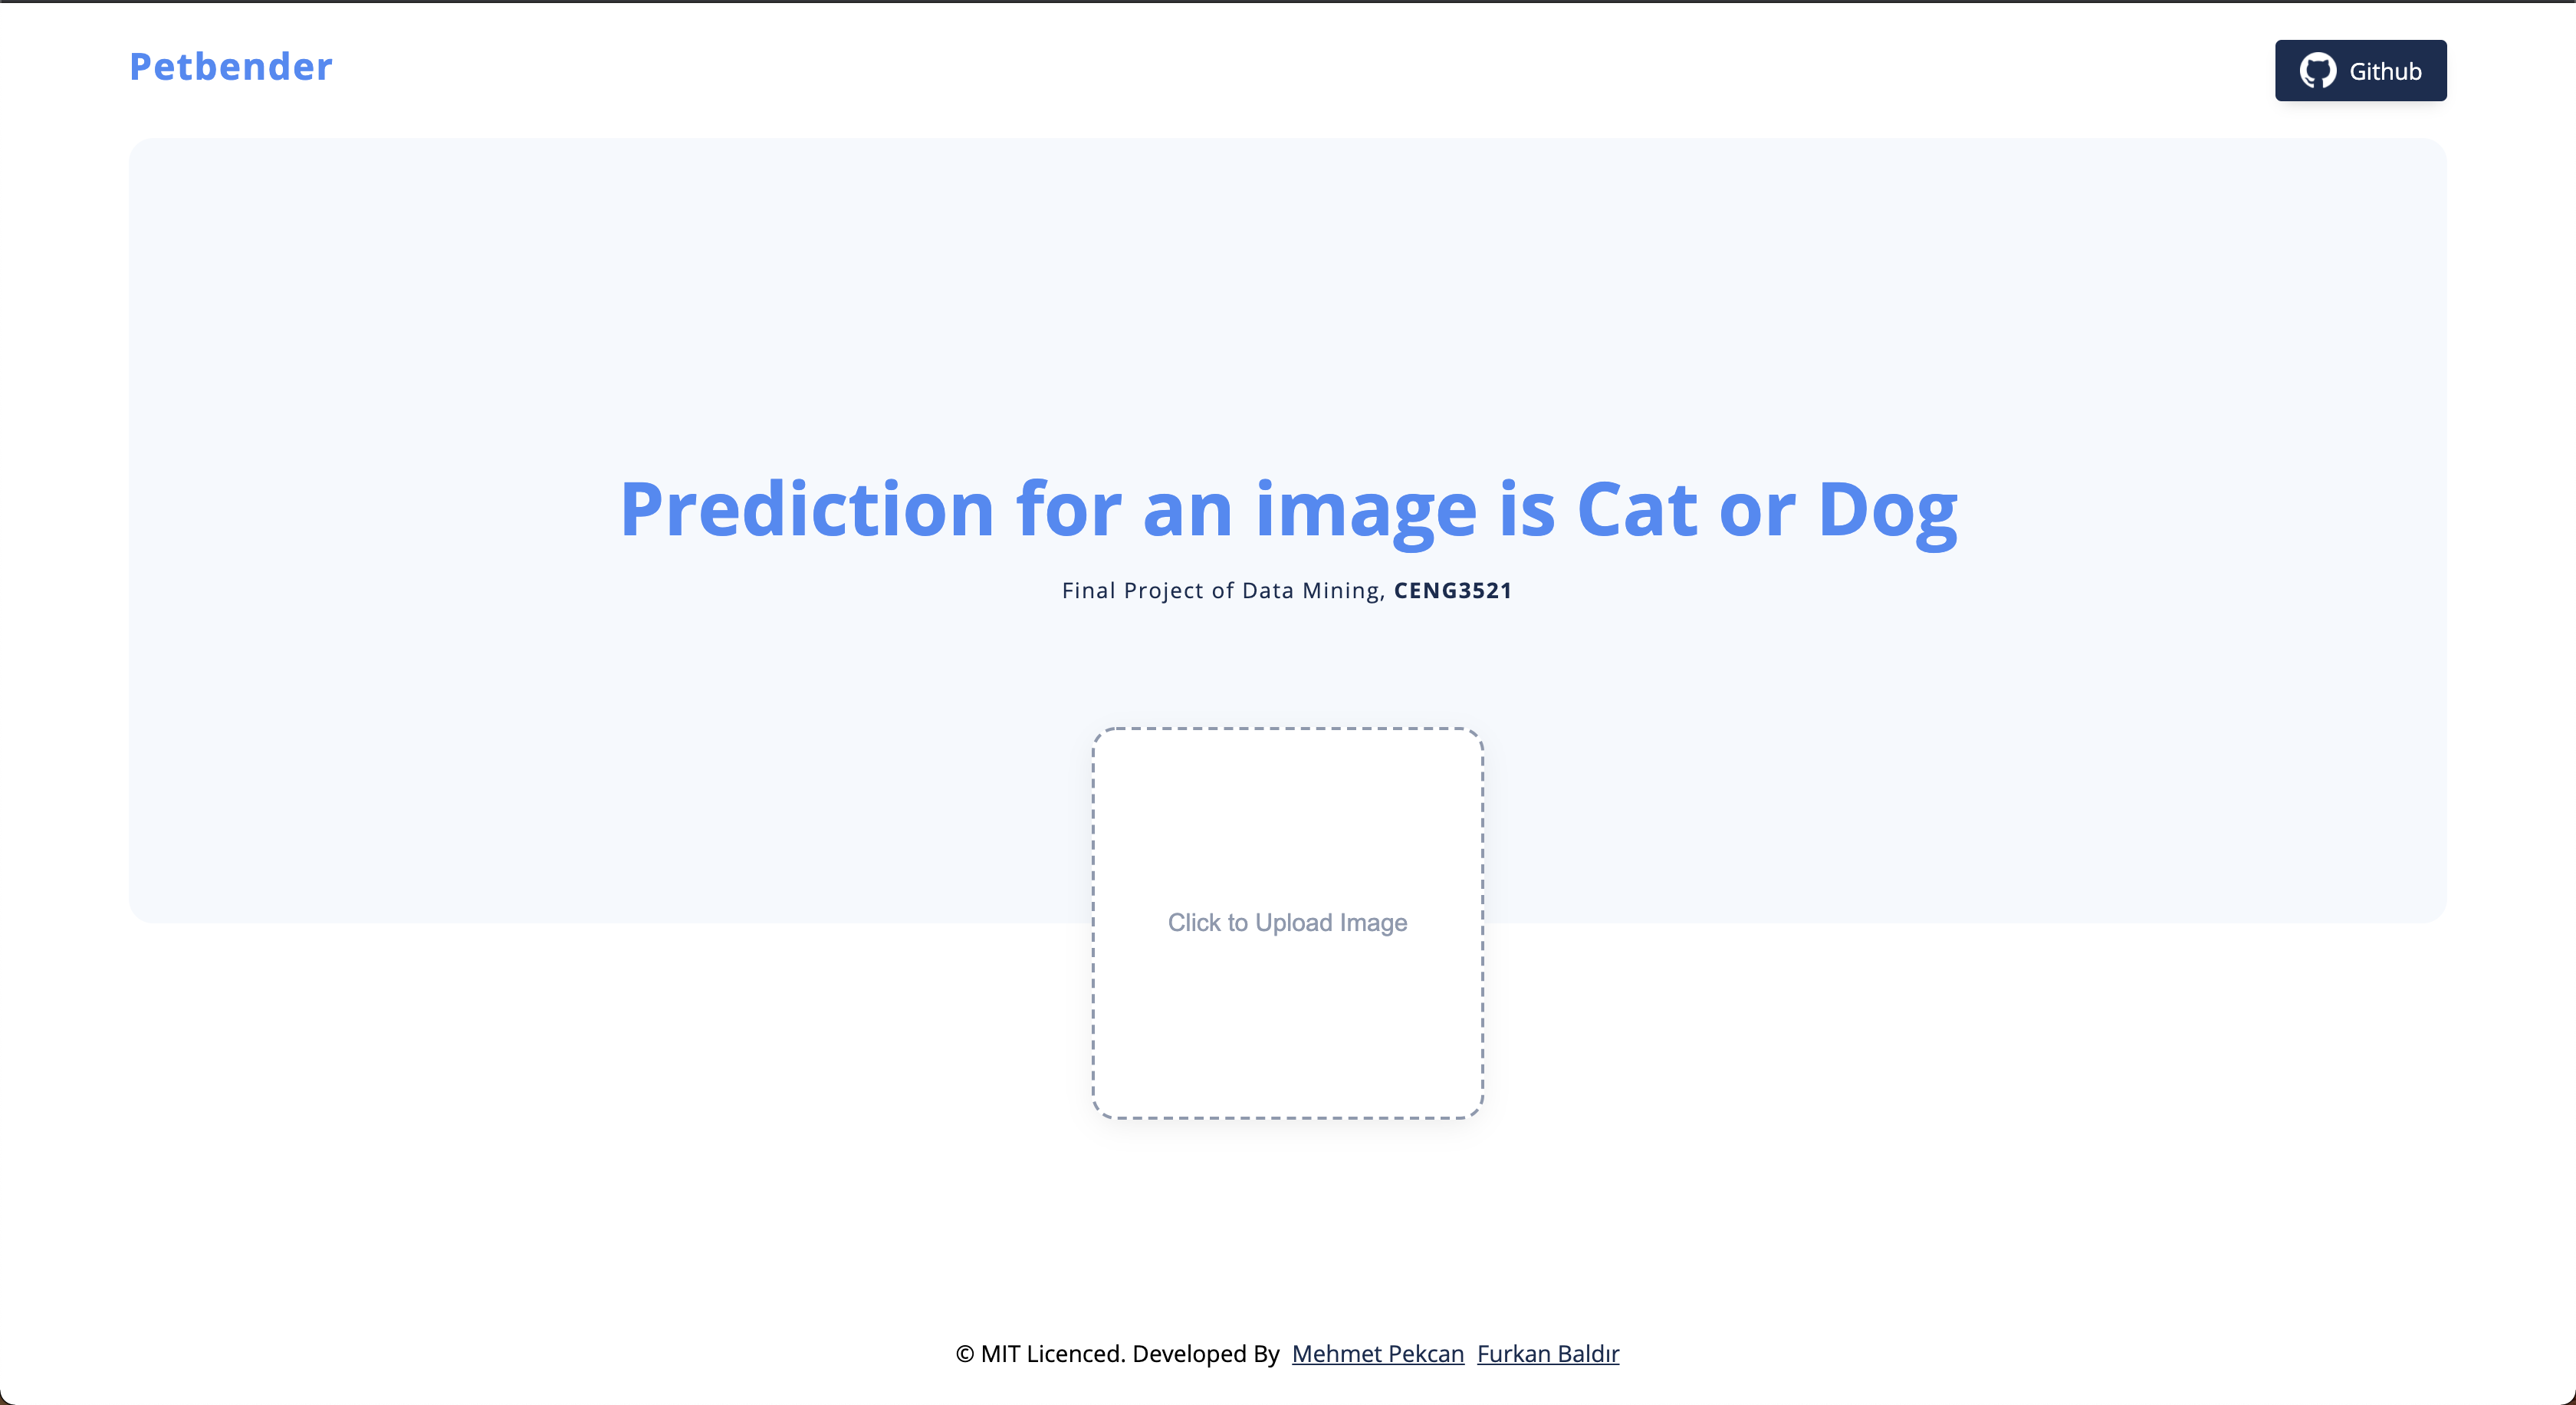
\includegraphics[scale=0.20]{init.png}
\caption{Main page of the web app}
\end{figure}

\begin{figure}[H]
\centering
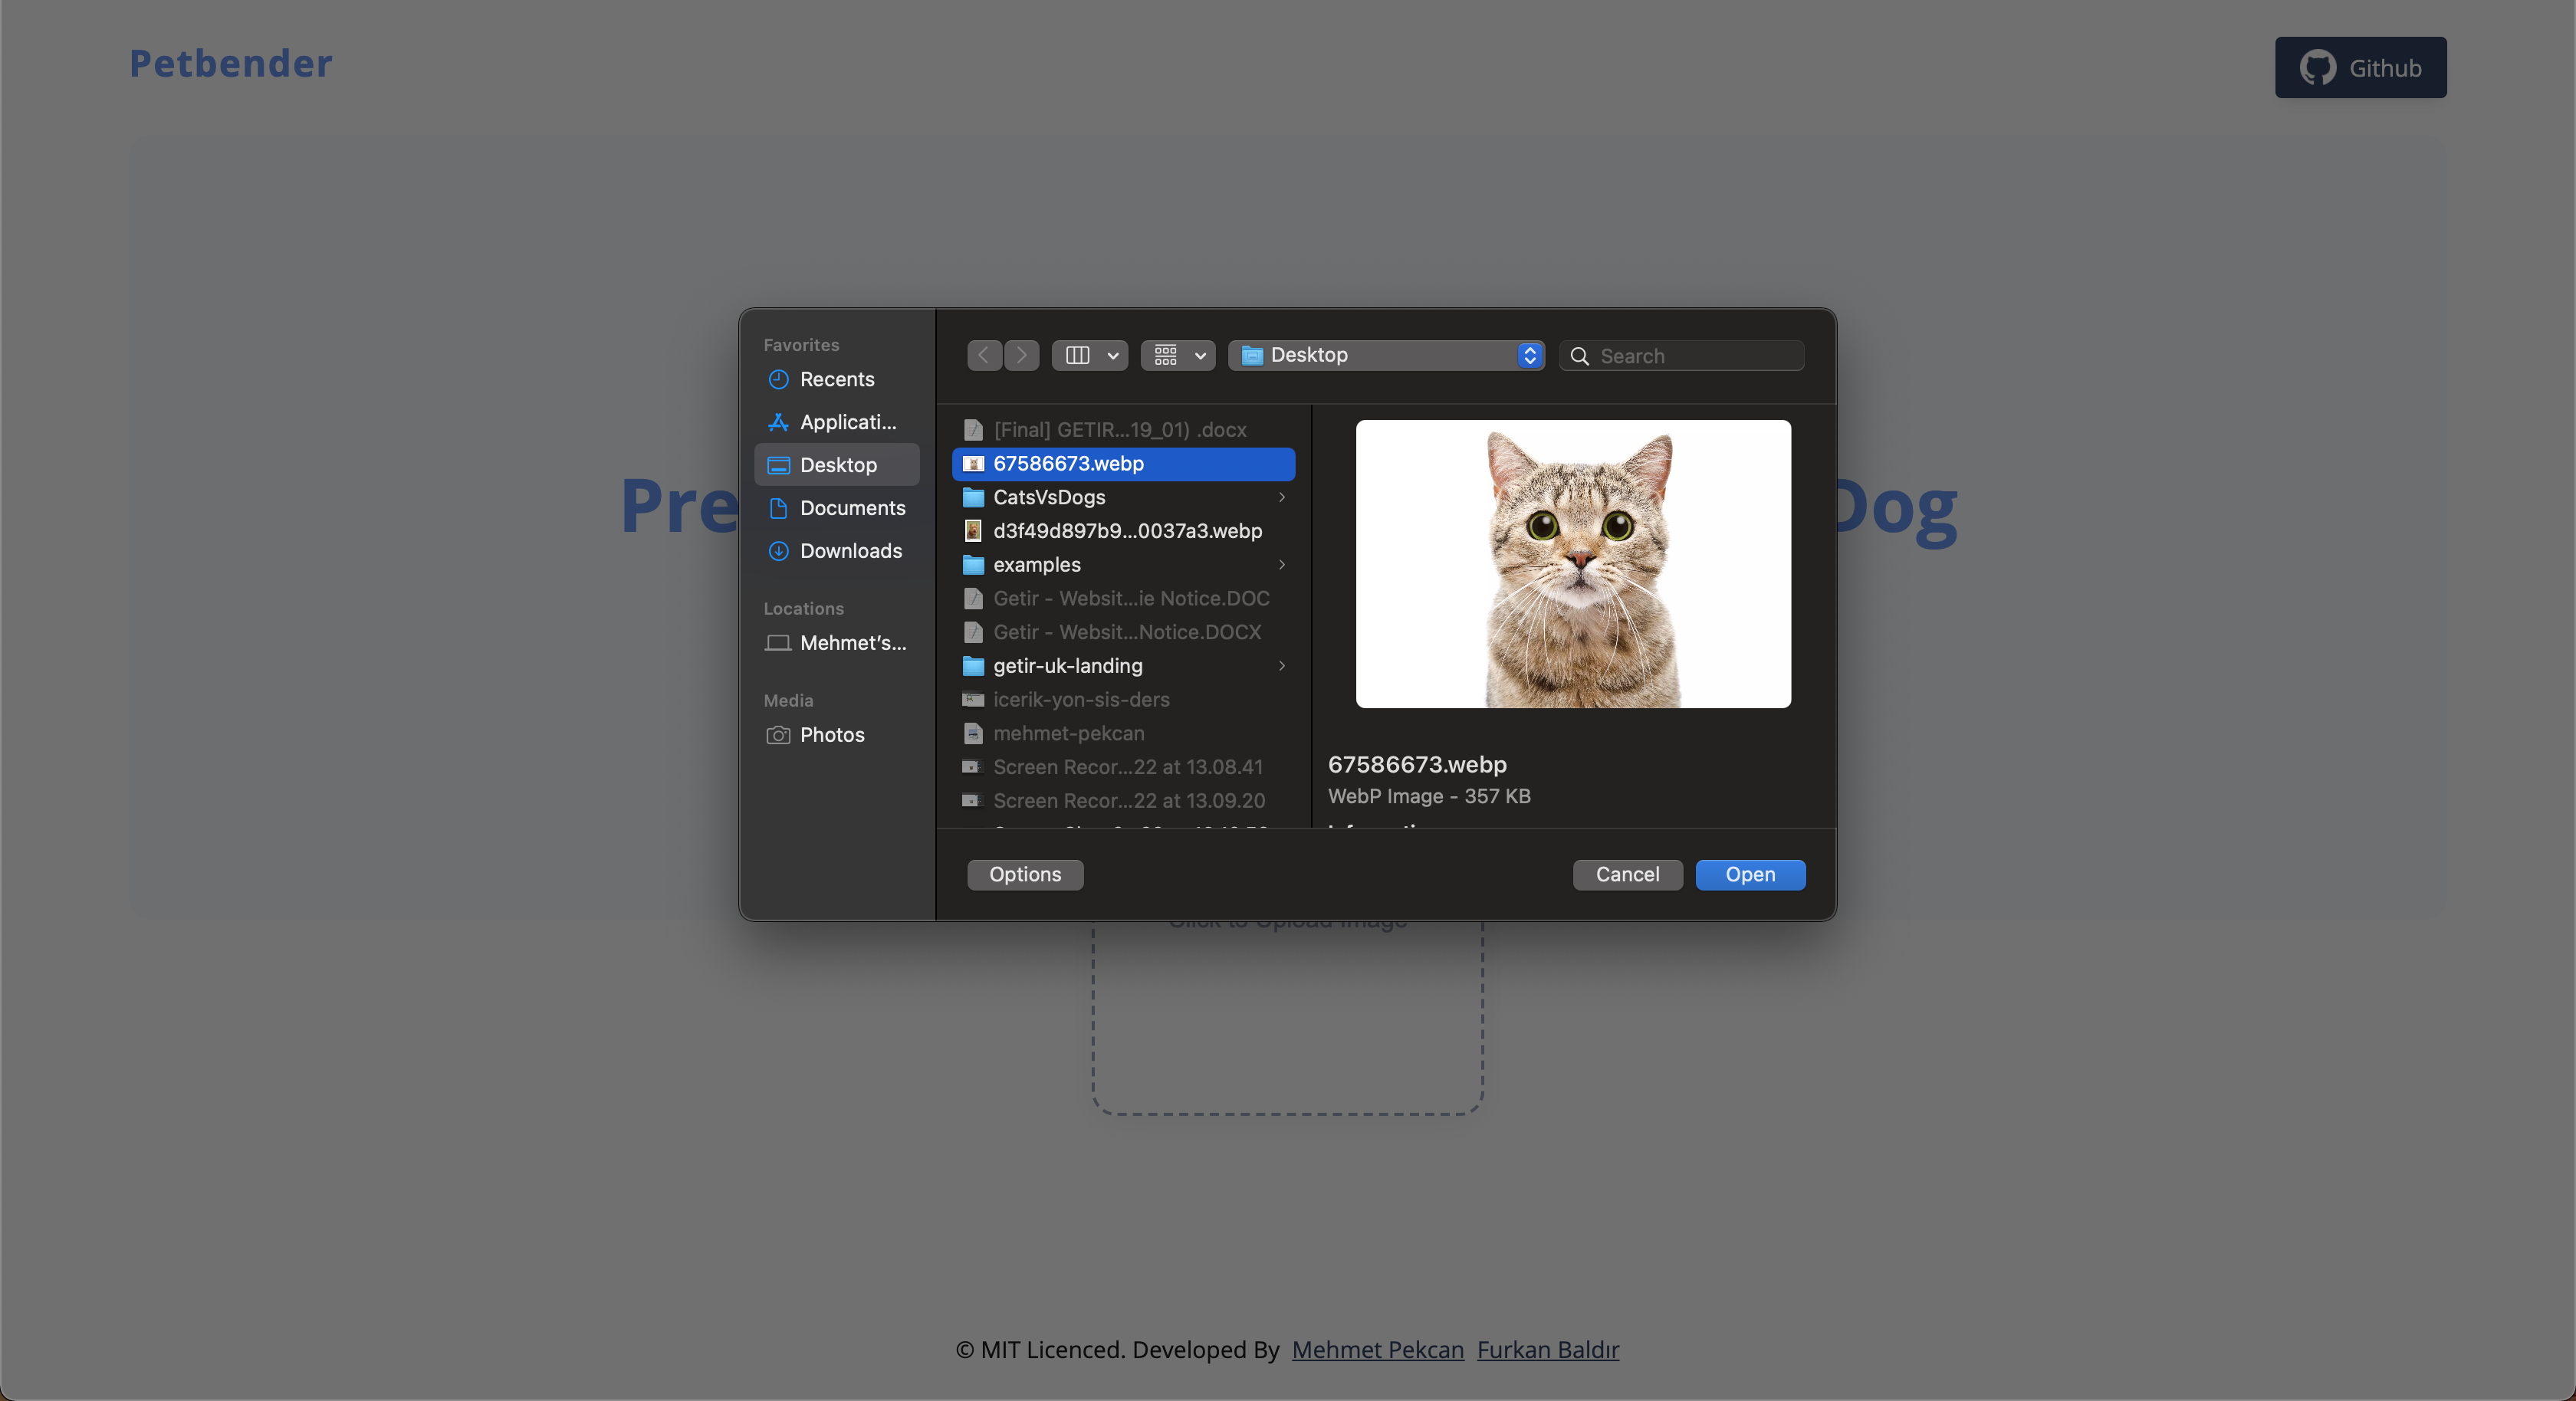
\includegraphics[scale=0.20]{load.png}
\caption{Choosing and uploading image}
\end{figure}

\begin{figure}[H]
\centering
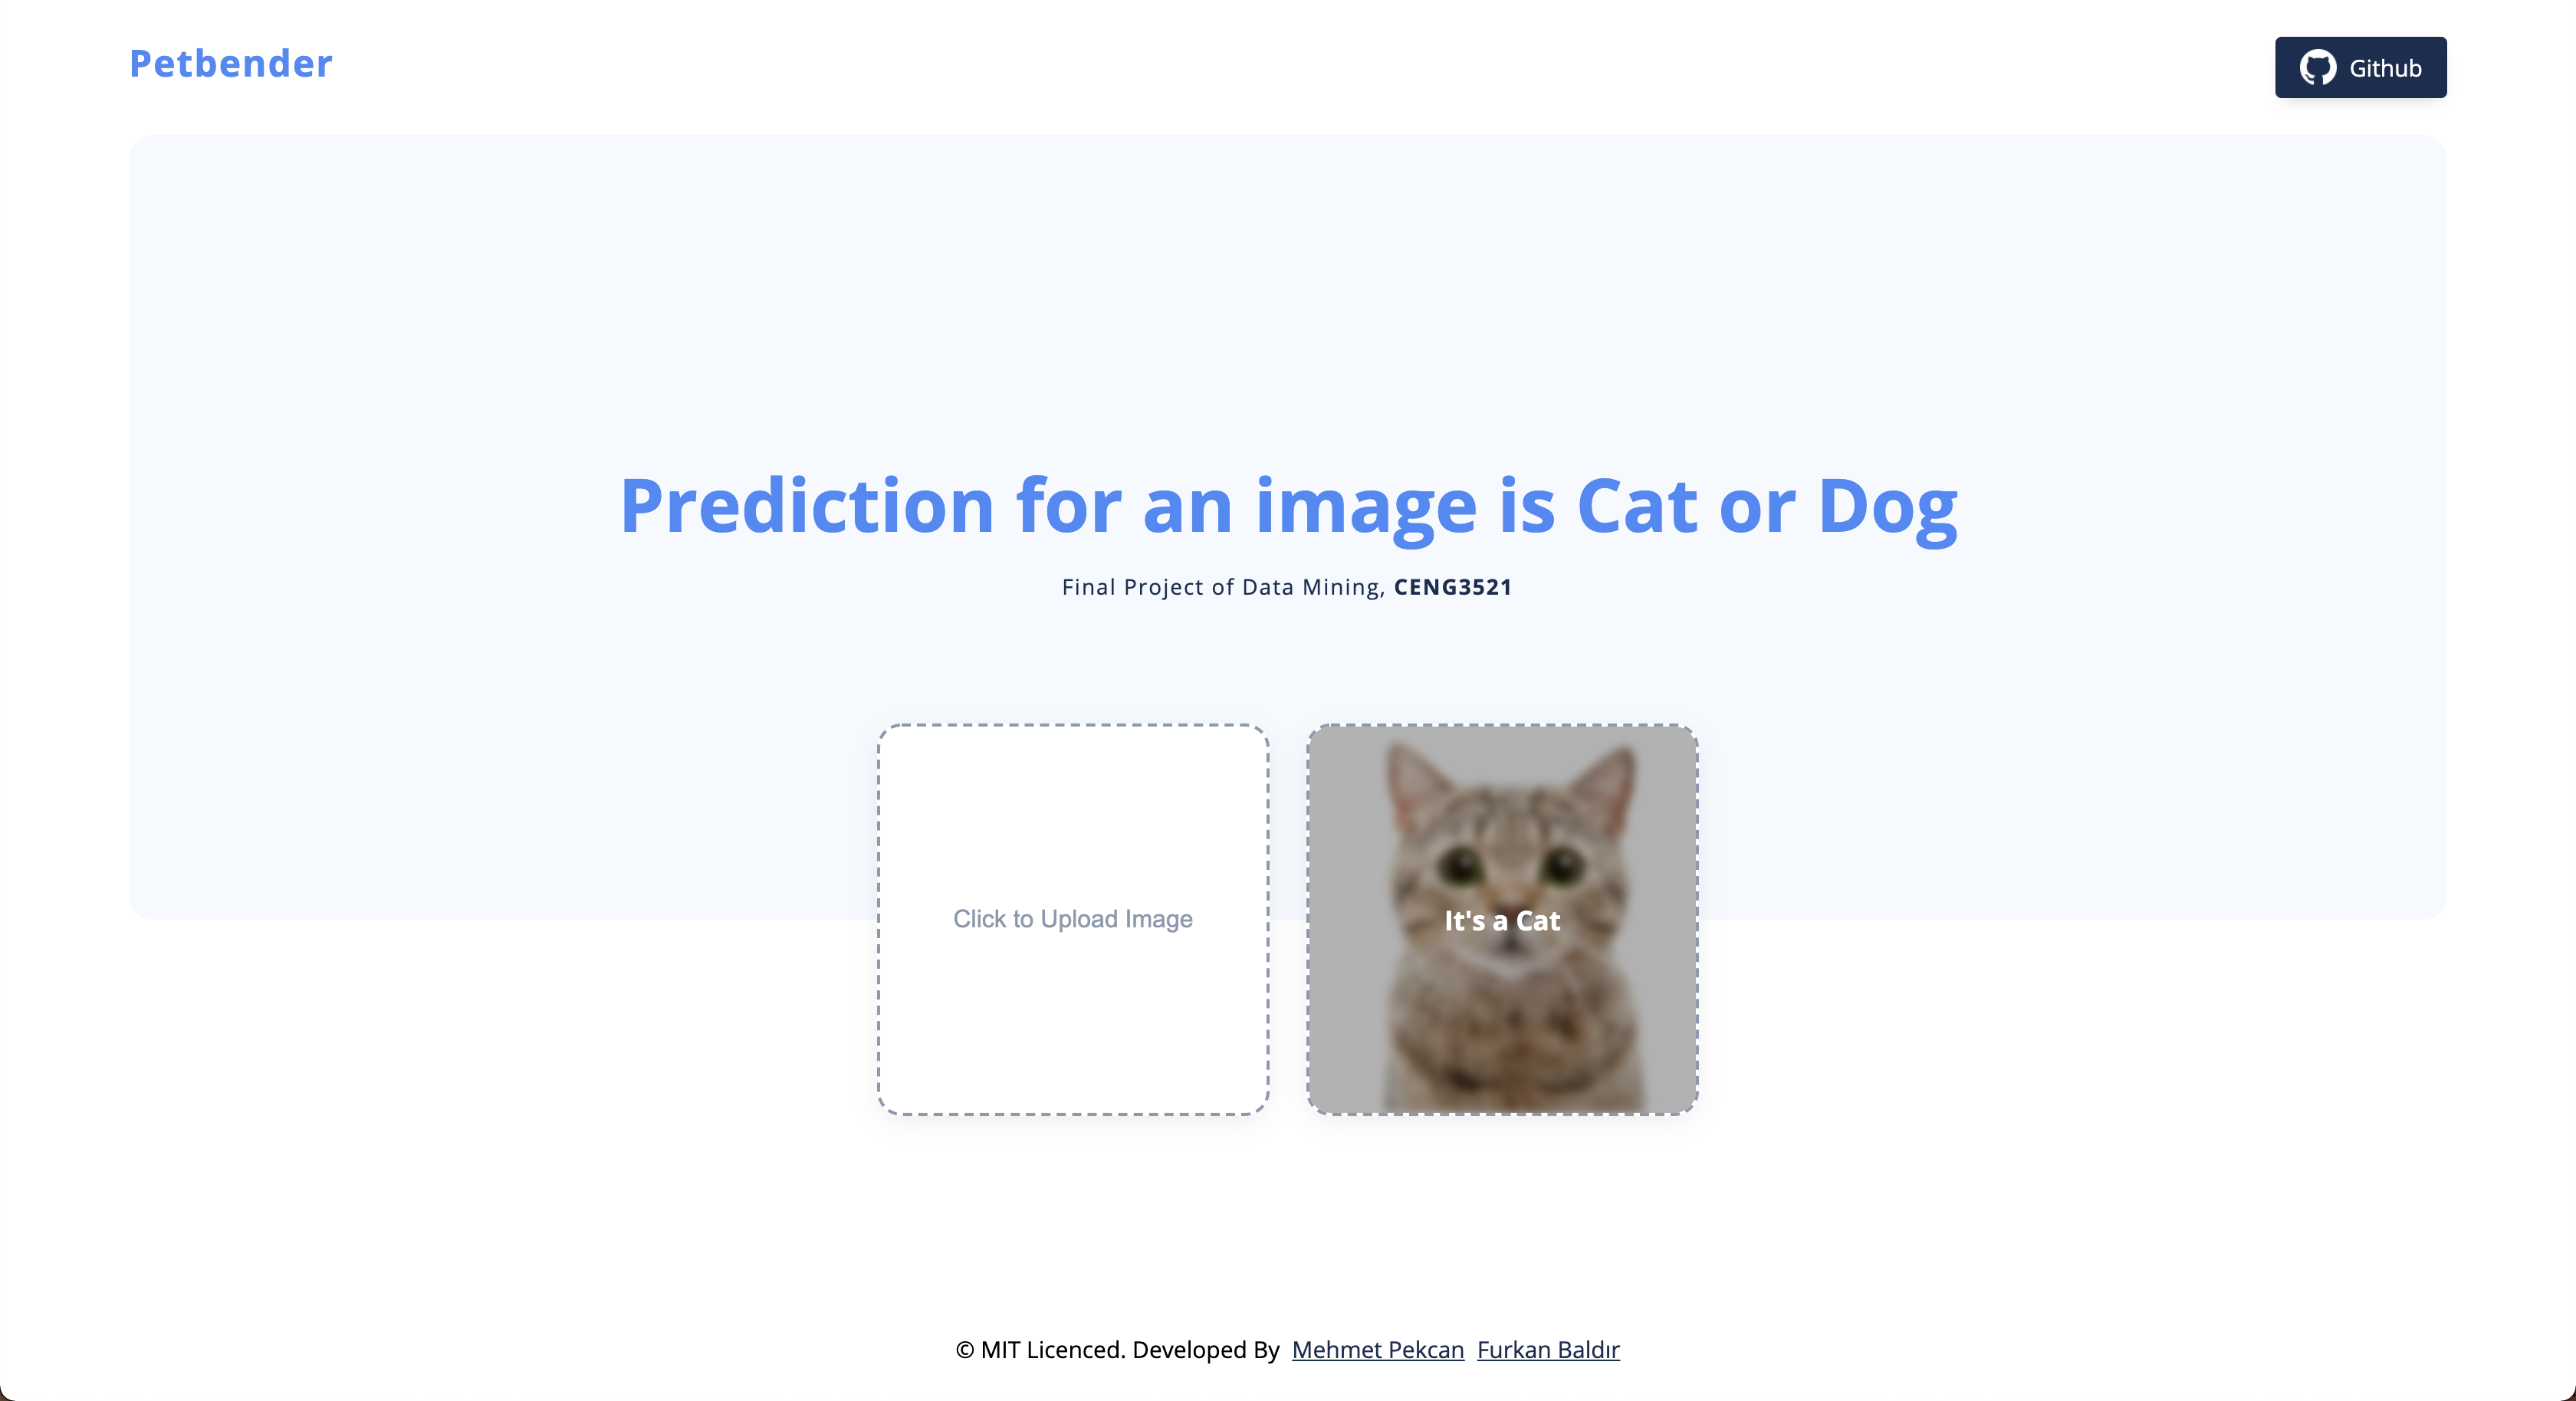
\includegraphics[scale=0.20]{loaded.png}
\caption{Showing the predicted class}
\end{figure}

\section{Results}
First of all, we have a project website click to go: \href{https://supremepanda.github.io/CatsVsDogs/}{CatsVsDogs}
\newline
\newline
In machine learning side, there are 2 results to mention:

\subsection{The Accuracy of Support Vector Machine Algorithm}
As we know, machine learning algorithms have less accuracy than deep learning algorithms to make image processing. That's why we didn't be in expectation to get very high accuracy. Our goal is to calculate how much accuracy we can get with the machine learning algorithm. As we said, we have test dataset to calculate accuracy with using \boldsymbol{predict\_with\_test\_data()} from \boldsymbol{backend/predict.py} script. 
\newline
\newline
The accuracy: \boldsymbol{\%59}

\begin{figure}[H]
\centering
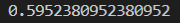
\includegraphics[]{accuracy.png}
\caption{Accuracy of model with test dataset}
\end{figure}



\subsection{Deployed Project Works Fine}
As we said, our web page is online on \href{https://supremepanda.github.io/CatsVsDogs/}{https://supremepanda.github.io/CatsVsDogs/}. You can upload an image, and you should wait the result which is cat or dog.
\newline
\newline
Note: Response may come a little late. The reason for this is that we benefit from free server services and as a result we have uploaded our project to a low speed server.

\section{Conclusion}
First of all, this project is an machine learning project to predict given image. For this work, Python handled  machine learning and API parts, Javascript handled frontend part of project.
\newline
\newline
This project has two main aim to solve:
\newline
\newline
Being a web application for users to predict given image.
\newline
Calculating accuracy of the machine learning algorithm.
\newline
\newline
As a result, this project works as a web application to predict given image as cat or dog. 
\end{document}